\documentclass{report}

\usepackage{amsmath}
\usepackage{bm}
\usepackage{graphicx}
\usepackage{tikz-cd}
\usepackage{amsfonts}
\usepackage{chngpage}
\def\ii{{\rm i}}


\newcommand{\re}[1]{\textcolor{blue}{[{\bf RE}: #1]}}
\newcommand{\cl}[1]{\textcolor{cyan}{[{\bf CL}: #1]}}


\DeclareMathOperator{\Li}{Li}
\DeclareMathOperator{\diag}{diag}
\DeclareMathOperator{\Arctan}{Arctan}
\DeclareMathOperator*{\argmax}{arg\,max}

\begin{document}
\title{Oscillon Dynamics in Classical\\ Scalar Field Theory}
\author{Chang Liu}
\maketitle

\tableofcontents

\chapter{Introduction}
\section{What is an oscillon?}
An oscillon is a spatially compact, temporally oscillatory, {\em long-lived} \re{usually non-exact - I think you can just say ``long lived solution'' - any analytic expression will be an approximation but the ``oscillon'' is the solution} solution to a non-linear wave equation. Mathematically speaking, given the standard wave equation in $d=1+D$ dimensions\footnote{In this thesis, we take the metric signature to be $\eta^{\mu\nu} = \diag(+1,-1,\ldots,-1)$}
\begin{equation}\label{wave}
  Du := \partial^2 u + V'(u) = 0
\end{equation}
with a non-linear potential $V(u)$, we define an oscillon solution to be a $C^\infty$ function that satisfies the following conditions:
\begin{enumerate}
\item For all fixed times $t$, the functions $u(t, x^i)$ have compact support along the spatial dimensions. This implies that $u(t,x^i)\to0$  when $x^i \to \infty$. \cl{I wanted to be precise when we talk about a mathematically defined object --- I think these definitions capture the necessary conditions for an oscillon solution?} \re{Fair enough. But rather than giving a condition on $u$, I would define this in terms of the total energy -- if the total energy of the configuration is finite and $u$ is asymptotically vanishing you don't care about how fast it vanishes; although you also need to stipulate that you are looking at the density $\rho-V_0$ since if $V_0 \ne 0$ then the total energy will diverge vanish, and that gives a condition on how fast $u$ must go to its asymptotic value}, 
\item For all fixed points $x^i$, the functions $u(t, x^i)$ are quasi-oscillatory and bounded in time.
\item $u(t,x^i)$ solves the non-linear wave equation (\ref{wave}) with a small radiation residual: $Du(t,x^i) \approx 0$. \cl{What I meant was, because the full solution to the non-linear eq.~would be oscillon+radiation, $Du(t,x^i)$ is only approximately zero, and if you look at the residual after applying the differential operator to the (approximate) oscillon solution, it will be a small out-ward radiation (ie.~solution to the linear wave eq).} \re{In terms of the mathematical definiton, I think the solution is just the solution -- this is a qualitative distinction, and need not form part of the definition -- at large distances there is a clear distinction between the outgoing radiation and the oscillon, but that will be fuzzy near the ``edge of the oscillon'' and it will not be critical to the discussion}
\end{enumerate}

Intuitively speaking, an oscillon is a spatially localized ``lump'' of mass\re{-energy} that oscillates around the zero-value plane (the hyper-plane $x^i=0$) \re{do you just mean it is located at the origin? if so that might be a more intuitive way to say it}. What makes oscillons interesting from a physics point of view is that for many non-linear potentials, oscillons are meta-stable: that is, although an oscillon \re{solution contains} outward radiations and \re{will} eventually decay, the time it takes to do so is significantly longer than the fundamental oscillation time-scale. \re{For the special case of} the sine-Gordon potential in 1 spatial dimension, oscillon solutions are exact and do not decay at all. This meta-stability makes oscillon solutions interesting in a wide range of physics phenomena.

Oscillons are studied in applied mathematics, cosmology, condensed matter physics, and other branches of physics. \re{Somewhere you need to cite all the examples of oscillons in physical systems} This Introduction will serve as a review of the vast corpus of relevant literature from different branches of mathematics and physics, \re{to provide a unified overview of the subject. } %in hoping to provide a unified view of the subject.

Before we begin we will clarify \re{terminology.} %as usage differsthe terminologies on this subject used across different branches in mathematics and physics: 
In applied mathematics, the term ``breather'' is synonymous \re{with} 
%to our term 
``oscillon'' \re{in the sense it is used here}. 
%They can be used interchangeably without any change in meaning. 
We will later use the phrase ``breathing behaviour'' to describe pulsating profiles in two-scale oscillons in subsequent chapters of this Thesis, \re{but will not the use the   term ``breather''}.

\section{Oscillons in the Applied Mathematics}
From an applied mathematics point of view, a wave equation can be classified into two categories: those that are exactly integrable \cl{I believe non-integrable equations generally don't have (exact) solutions?}\re{what I meant, is can you characterise this independently of whether you can find an exact solution}, and those that are not. The former class contains the standard constant-coefficient linear wave equation, and the sine-Gordon equation in 1D:
\begin{equation}
  \partial^2_t u - \partial^2_x u + \sin u = 0
\end{equation}
with the 1D sine-Gordon potential $V(u) = 1-\cos u$. Other non-linear potentials (including sine-Gordon in 2 or more spatial dimensions) are not integrable.

It can be shown that the linear wave equation does not support meta-stable oscillon solutions \cite{Copeland:1995fq}. 
%Therefore 
This section will first review oscillon solutions to the integrable 1D sine-Gordon equation and then will then look at oscillons in the more general non-integrable case. \re{suggested rewording}

\subsection{General Solutions to the 1D Sine-Gordon Equation}

\re{I think you want to give some specific examples here, and in the previous subsection -- a couple of plots, or an animation, as well as the physical systems where they show up}

The sine-Gordon equation was first introduced in the 19th century by Edmond Bour, as the Gauss-Codazzi equation for surfaces of constant curvature $-1$ in 3-space \cite{bour}. \re{What does this equation describe?} It was then realized that the 1D sine-Gordon equation supports the so-called ``kink'' and ``anti-kink'' solutions, which can interact non-linearly \cite{Perring:1962vs} and are termed ``solitons'', as they behave just like particles when they scatter against each other and retain their original shape without distortion. This generated great interest in understanding the general solitonic solutions to the 1D sine-Gordon equation in the 1970s, and lead to the development of the inverse scattering transform as a general method of integrating certain non-linear partial differential equations \cite{SAPM:SAPM1974534249}. \re{Solitons are originally known from water wave solutions, I think (on a plane so can't check!) so you should make this connection.} 

The most comprehensive review of the inverse scattering transform is the book \cite{ablowitz} by Ablowitz, one of the inventors of this method. We also note a few shorter, more accessible introductions to the topics of integrable systems, solitons and inverse scattering transform in \cite{Aktosun2009, spiro, intsys}.

Based on the inverse scattering transform, it is possible to encode all general solitonic solutions to the 1D sine-Gordon solution into a ``matrix'' form. This ``matrix'' method takes an $n\times n$ matrix along with a set of ancillary $n$-dimensional vectors as input and generates a $n$-soliton. This is indeed the starting point of our construction of the two-scale oscillon. For a detailed description of this method, see the original paper \cite{:/content/aip/journal/jmp/51/12/10.1063/1.3520596}. There is also a shorter talk on this subject \cite{sgtalk}.

Another method of generating the solitonic solutions to the 1D sine-Gordon equation is the B\"acklund transformation \cite{Dodd499, hietarinta1997introduction, Cuenda20111047}, which is a non-linear generalization of the super-position principle of the linear wave equation. However, we note that the B\"acklund transformation can only generate \emph{solitonic} solutions, while the inverse scattering transform can generate both solitonic and radiative solutions, and combinations thereof.

\subsection{Generalizations of the sine-Gordon Equation}
We briefly mention some \re{ {\em of the possible} these words not needed} generalizations of the sine-Gordon equation that were studied in the literature. Some of these generalizations are exactly integrable, while others are not. We start with the exactly integrable cases and move on to the non-integrable ones.

\subsubsection{Exactly integrable cases}
\re{A generalization of the sine-Gordon equation  is} \cite{1751-8121-43-10-105204}
\begin{equation}
  u_{tx} = (1+\nu \partial^2_x)\sin u
\end{equation}
where $\nu$ is a real parameter. For $\nu<0$, this equation is exactly integrable and can be shown to have \re{novel} solitonic solutions in \cite{1751-8121-43-10-105204}  where %it was also shown that this form of generalization of the sine-Gordon equation supports a novel type of solitons where 
the smaller solitons travels faster than the larger soliton.

\medbreak
Another  generalization of the sine-Gordon equation is the vector sine-Gordon equation:
\begin{equation}\label{vectorsg}
  \partial_t\left(\frac{\bm{\alpha}_x}{\beta}\right) = \bm{\alpha}
\end{equation}
where $\bm{\alpha}$ is a $n$-dimensional real vector field and $\beta = \sqrt{1 - \langle\bm{\alpha},\bm{\alpha}\rangle}$. We require $\langle\bm{\alpha},\bm{\alpha}\rangle\le1$ so that $\beta\in\mathbb{R}$. Taking $n=1$ and $\alpha = \sin \theta$ reduces (\ref{vectorsg}) to the standard 1D sine-Gordon equation $\theta_{tx} = \sin \theta$.

This equation is also exactly integrable. By using a Lax-pair based approach called the ``dressing method'' which is similar to the inverse scattering transform \re{Ref.~}\cite{Mikhailov201653} \re{shows} it is possible to obtain similar solitonic solutions as in the case of 1D sine-Gordon equation.

\subsubsection{Non-integrable cases}
A different direction in generalizing the sine-Gordon equation is to add perturbation to it. For a general perturbation, this usually makes the equation non-integrable.  \re{Ref.~}\cite{PhysRevB.85.134525} investigated the radiative annihilation of a soliton and an anti-soliton in the following perturbed, coupled vector sine-Gordon equation:
\begin{equation}
  \partial^2_x\phi_i=\sum_j \mathbf{A_{ij}} \left[\partial^2_t \phi_j +\alpha \phi_j +\sin \phi_j - \gamma\right]
\end{equation}
where $\alpha$ is the viscous damping parameter and $\gamma$ is the driving term. This equation is not integrable, and therefore only numerical analysis was performed. It was shown in \cite{PhysRevB.85.134525} that this equation supports solitonic solutions, and soliton-anti-soliton pairs will annihilate even in the absence of perturbations, which is not the case in plain 1D sine-Gordon equations.  \re{Ref.~}
\cite{RevModPhys.61.763} provided a comprehensive review of the method inverse scattering transform when applied to nearly integrable systems which are exactly integrable equations perturbed by certain treatable forms of perturbation.

\medbreak

A final generalization to the sine-Gordon equation is to consider a slight deformation of the sine-Gordon potential. \cite{Ferreira2011} investigated the following potential
\begin{equation}\label{deformed}
  V(\phi, n) = \frac{2}{n^2} \tan^2 \phi \left( 1 - \left|\sin\phi\right|^n \right)^2
\end{equation}
which reduces to the plain sine-Gordon equation when $n=2$. \cite{Ferreira2011} considered the case $n=2+\epsilon$, where $V$ can be expanded around the exact sine-Gordon potential assuming $\epsilon$ is small. This leads to the concept of ``quasi-integrability'', which allows one to obtain solitonic solutions and their asymptotic conservation laws. \cite{Ferreira2011} also demonstrated numerically that (\ref{deformed}) supports long-lived oscillons and other solitonic solutions.

\subsection{General Non-linear Potentials}
In general, one does not expect any form of integrability for a general non-linear wave equation. However, for certain special cases one can nonetheless construct oscillon solutions directly. An example is the swaying oscillons in the signum-Gordon model \cite{Arodz:2011zm}:
\begin{equation}
  V(\phi)=\left|\phi\right|
\end{equation}

It can be shown \cite{Arodz:2011zm} that this type of potentials support the ``swaying'' oscillon solutions where the center of oscillon sways in a fixed interval periodically while the overall size of the oscillon remains strictly constant. These oscillons are exact analytic solutions.

\medbreak

For general non-linear potentials, there are two broad categories of approaches in terms of understanding the properties of oscillons: non-perturbative methods, and numerical methods. We will discuss them separately.

\subsubsection{Non-perturbative methods}\label{nonpert}
\begin{figure}\centering
  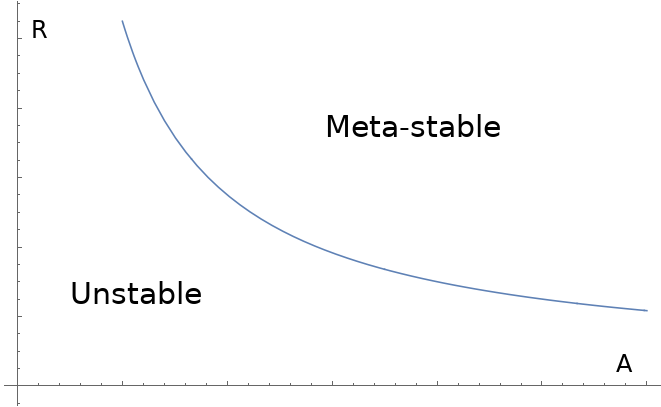
\includegraphics[width=0.5\textwidth]{plot/stability.png}
  \caption{Typical stability map starting from Gaussian initial profiles with amplitude $A$ and radius $R$.}
  \label{stability}
\end{figure}

The general non-perturbative methods for analyzing oscillon dynamics are described in detail in \cite{Copeland:1995fq, PhysRevD.80.125037, Gleiser:2008ty}. The idea is to expand the potential in power series and integrate each order in the power series separately. We will later (in Chapter 2) point out that this method has serious limitations as it only apples to finite order polynomial potentials. It will fail on, for instance, the axion-monodromy potential. Nonetheless, it is possible to establish some important properties of oscillons using this series expansion technique. The main results are:
\begin{enumerate}
\item The meta-stability of oscillons is due to the fact that the non-linear potential acting as the ``restoring force'' does not increase linear so that out-ward radiation is greatly suppressed. In a linear theory, an initial oscillon profile will decay rapidly and no meta-stable oscillons can be formed.
\item Starting from a Gaussian initial profile $\phi(0,r)=A\exp(-r^2/R^2)$, one can obtain a stability map which typically looks like \ref{stability}, which has a distinctive region in the parameter space where oscillons are meta-stable. Outside this region, the oscillons decay rapidly and are not stable. We will later see that in our numerical study of the axion-monodromy oscillons, the oscillons that live near the stable-unstable separation have strong breathing modes.
\item Using the series expansion technique, one may establish an analytic expression for the decay rate of oscillons (eq.~(49) in \cite{PhysRevD.80.125037}. It can also be argued that there is an attractor point in the configuration space to which oscillons tend, by minimizing the effective potential obtained from the series expansion.
\end{enumerate}

Additionally, it can be established \cite{Mukaida:2016hwd} that the longevity of oscillons can be understood as the result of an effective theory with an approximate global $U(1)$ symmetry. This approximate $U(1)$ symmetry will lead to an approximate number conservation which will lend to the extreme longevity of oscillon configurations. Oscillon decay can then be understood as the breaking of this $U(1)$ symmetry via number-conservation violating processes. Both this study and the previous non-perturbative method are consistent in terms of establishing the fact that oscillon longevity is a dynamic process, where the longer time-scale appears dynamically, rather than as a parameter of the theory.

\subsubsection{Numerical methods}
In all of the studies listed in the previous subsection, the analytical methods are accompanied with numerical studies to confirm their findings. We also note several additional numerical studies dedicated to study certain types of oscillons.

\cite{Salmi:2012ta} studied the power spectrum of the field oscillation at the center of the oscillon, and found that at least for the oscillons that were being studied, the power spectrum has a distinctive shape (see Fig.~6 of \cite{Hindmarsh:2006ur}). We will later use the same method to study the power spectrum of two-scale oscillons and find that the power spectrum has a different shape.

\cite{Hindmarsh:2006ur} studied oscillons in 2 spatial dimensions using a similar method as in \cite{Salmi:2012ta}. What is noteworthy in this study is that it found breathing modes in 2D sine-Gordon oscillons. These breathing modes are the main focus of this Thesis. We will confirm the studies done in this paper and provide an analytic characterization of the breathing modes.

\section{Oscillons in the Early Universe}\label{litrev:cosmo}
In string inflations \cite{stringInflationBook, McAllister:2008hb, Silverstein:2008sg, Flauger:2009ab}, a natural candidate of the inflaton field is the axion-monodromy potential:
\begin{equation}
  V(\phi) = \frac{m^2M^2}{2\alpha} \left[\left(1+\frac{\phi^2}{M^2}\right)^\alpha -1\right]
\end{equation}

It is established in \cite{Amin:2010dc, Amin:2011hj} that parametric resonance provides a natural and dynamical process of generating axion-monodromy oscillons in the (p)re-heating stage of the inflationary universe. The parametric resonance can be analyzed using Floquet theory and the existence of an oscillon dominated phase is confirmed by numerical simulation of the post-inflation universe, using PSpectRE \cite{Easther:2010qz}.

The analytic study of oscillons in an expanding universe is done in \cite{Amin:2010jq}, where it also found a new class of ``flat-top'' oscillons in the $\phi^6$ theory. The detailed Floquet analysis can be found in \cite{Amin:2010dc}.

\section{Oscillons in Other Physical Systems}
Oscillons are also observed in many condensed matter systems, including Bose-Einstein condensates \cite{umbanhowar1996localized}, nonlinear optics \cite{Copeland:2014qra}, and vibrated granular materials \cite{Tsimring:1997zz}. We also note that in applications to nonlinear optics, the sine-Gordon equation is solved in a different boundary condition than what we are using here, namely they use periodic boundary condition for both space and time \cite{JAWORSKI1982427, 0305-4470-15-10-015}. \cite{JAWORSKI1982427, 0305-4470-15-10-015} discussed possible oscillon-like solutions in this type of boundary conditions.

\chapter{Comments on the Series Expansion Technique for General Nonlinear Potential}\label{nonpertprob}
The ``series expansion'' technique refers to the non-perturbative method of treating oscillon dynamics in a general non-linear potential, described in \cite{PhysRevD.80.125037, Gleiser:2008ty}. The idea of this method is to expand the potential $V(\phi)$ into a power series around the vacuum $\phi_0$ which we assume to be $0$:

\begin{equation}
  V(\phi)=\sum_{n=0}^\infty \frac{g_n}{n!}\phi^n
\end{equation}

We then substitute the Gaussian ansatz
\begin{equation}
  \phi(r,t) = A(t) \exp\left(-\frac{r^2}{R^2}\right)
\end{equation}
into the full Lagrangian
\begin{equation}\label{lagfull}
    L = \frac{2\pi^{d/2}}{\Gamma(d/2)}\int r^{d-1}\,\mathrm{d}r\left[\frac{1}{2}\dot{\phi}^2 -
      \frac{1}{2}\left(\frac{\partial\phi}{\partial r}\right)^2-V(\phi)\right]
\end{equation}
and integrate out the radial part, so that the dynamics becomes that of a single variable function $A(t)$:
\begin{equation}
  L= \left(\frac{\pi}{2}\right)^{d/2}R^d\left[\frac{1}{2}\dot{A}^2 - V_{\rm eff}(A)\right]
\end{equation}

This $A(t)$ function will then have a classical motion in an effective potential $V_{\rm eff}$, where
\begin{equation}\label{effpot}
  V_{\rm eff}(A) = \frac{A^2d}{2R^2} +
  \sum_{n=0}^\infty \frac{g_n}{n!}\left(\frac{2}{n}\right)^{d/2} A^n
\end{equation}

This is a valid approach for polynomial potentials (namely, potentials that are truncated power series). However, we will demonstrate here that this approach fails for more complicated potentials which have an infinite power series expansion and a finite radius of convergence. An example is the axion-monodromy potential in inflation cosmology:
\begin{equation}
  V(\phi) = \frac{m^2M^2}{2\alpha}\left[\left(1+\frac{\phi^2}{M^2}\right)^\alpha-1\right]
\end{equation}
where $\alpha=1/2$.

We note that a trivial re-scaling allows us to set
\begin{equation}
  m=M=1
\end{equation}
Therefore we will take
\begin{equation}\label{V}
  V(\phi)=\sqrt{1+\phi^2}-1
\end{equation}

In what follows, we will show that a naive application of the series expansion technique to the axion-monodromy potential does not give the desired result --- the stability criterion predicts that oscillons are unstable and therefore cannot be formed, while from numerical simulations we have clearly seen oscillon formations in both the post-inflationary universe and the plain numerical integrator.

To start, we expand (\ref{V}) into power series:
\begin{equation}\label{Vexpand}
  V(\phi)=\sum_{n=1}^\infty\frac{\alpha(\alpha-1)\cdots(\alpha-n+1)}{n!}\phi^{2n}
\end{equation}
and note that it has a finite radius of convergence $r=1$. Substituting (\ref{Vexpand}) into (\ref{effpot}), we have
\begin{equation}\label{Veff}
  V_{\rm eff}(A)=\frac{A^2d}{2R^2} + \sum_{n=1}^\infty\frac{\alpha(\alpha-1)\cdots(\alpha-n+1)}{n!}
  \left(\frac{1}{n}\right)^{d/2}A^{2n}
\end{equation}
Both sums in (\ref{V}) and (\ref{Veff}) have radius of convergence 1 and are holomorphic within their radius of convergence. In order to evaluate $V_{\rm eff}(A)$ for $A>1$, we note that the effective potential $V_{\rm eff}$ is defined as an integral in (\ref{lagfull}), and is therefore analytic in its domain. This allows us to analytically continue the second sum to obtain a meromorphic function in $\mathbb{C}$. We will denote the function thus obtained as $F(z)$. In other words,
\begin{equation}\label{VeffFz}
  V_{\rm eff}(A) = \frac{A^2d}{2R^2} + F(A)
\end{equation}

To solve for $F(z)$ explicitly, note for a start that for $d=2$, differentiate $F(z)$ gives
\begin{equation}
  F'(z)=\sum_{n=1}^\infty\frac{\alpha(\alpha-1)\cdots(\alpha-n+1)}{n!} \cdot 2 z^{2n-1}
\end{equation}
Therefore we have, for $d=2$,
\begin{equation}
  F'(z)=\frac{2}{z}\left[\sqrt{1+z^2}-1\right]
\end{equation}
Integrating this we have, assuming suitable branch cut,
\begin{equation}
  F(z) = 2 \left(\sqrt{z^2+1}-1-\log \frac{1+\sqrt{z^2+1}}{2}\right)
\end{equation}

We now substitute this expression for $F(z)$ into (\ref{VeffFz}), and obtain the final form of the effective potential for $d=2$:
\begin{equation}
  V_{\rm eff}(A) = \frac{A^2}{R^2} + 2 \left(\sqrt{A^2+1}-1-\log \frac{1+\sqrt{A^2+1}}{2}\right)
\end{equation}

The stability criterion in \cite{Gleiser:2008ty} states that the region where $I(A,R) = V''_{\rm eff}(A)<0$ gives meta-stable oscillon configurations. However, evaluating $V''_{\rm eff}(A)$, we have
\begin{equation}
  V''_{\rm eff}(A) = 2 \left(\frac{1}{1 + A^2 + \sqrt{1 + A^2}} + \frac{1}{R^2}\right)
\end{equation}
which is positive definite. Therefore, the stability criterion in \cite{Gleiser:2008ty} will predict no stable oscillons, which contradicts the findings we have in our numerical simulations.

Note that this procedure is applicable for all $d$ even. Set $d=2p$, differentiating $F(z)$ once gives
\begin{equation}
  \frac{z}{2}D_z F = \sum_{n=1}^\infty\frac{\alpha(\alpha-1)\cdots(\alpha-n+1)}{n!} \frac{1}{n^{p-1}} z^{2n}
\end{equation}
where $D_z$ denotes differentiating with respect to $z$. Differentiating $F(z)$ $p$ times therefore gives
\begin{equation}
  \left(\frac{z}{2}D_z\right)^p F = V(z) = \sqrt{1+z^2}-1
\end{equation}
Integrating the equation above then gives the explicit form of $F(z)$, once we take care of integration constants and branch cuts.

Another method of obtaining the same result is to evaluate the integral in (\ref{lagfull}) directly. In other words, if one substitutes the Gaussian ansatz into the full Lagrangian (\ref{lagfull}), one is faced with the evaluation of the following integral:
\begin{equation}\label{intE}
  E(\lambda) = \int^{+\infty}_0 \left[\sqrt{1+\lambda\exp(-r^2)} -1\right]r^{d-1}\,{\rm d}r
\end{equation}
where $\lambda \ge 0$.% The problem with using the series expansion method in Sicilia's paper directly for our case is that the function $\sqrt{1+\lambda z}$ has a singularity at $z=-\lambda^{-1}$, and when $\lambda$ goes above 1, the integration will hit the radius of convergence and therefore render the series expansion invalid.

%What I did previously was to note that $I(\lambda)$ is an analytic function of $\lambda$ (because it is an integral of an analytic function), and by the uniqueness of analytic functions, we can just evaluate $I(\lambda)$ for $\lambda < 1$, and the $\lambda > 1$ part will automatically come out from the $\lambda < 1$ expression.

%This is correct, but is totally useless, because we can evaluate $I(\lambda)$ directly (for some cases)!

For $d=2$, $E(\lambda)$ evaluates to
\begin{equation}
  \begin{split}
  E(\lambda) &= \int^{+\infty}_0 \left[\sqrt{1+\lambda \exp(-t)} -1\right]\,{\rm d}t\\
  &= -2\sqrt{1+\lambda\exp(-x)} + 2\log\left[1+\sqrt{1+\lambda\exp(-x)}\right]\Big|^{+\infty}_0\\
  &= 2\left(\sqrt{1+\lambda} -1 -\log\frac{1+\sqrt{1+\lambda}}{2}\right)
  \end{split}
\end{equation}
which is consistent with the result using analytic continuation.

\bigbreak

For odd $d$ we can numerically evaluate the integral (\ref{intE}) and obtain the same result that $I(A,R)$ is positive definite, which contradicts the findings in both stand-lone numerical integrator and the PSpectRE simulations. In evaluating $I(A,R)$ (or equivalently, $E(\lambda)$), it is useful to rewrite the $F(z)$ function into a different form, by employing the technique of fractional derivative and integration. Defining
\begin{equation}
  (D^\alpha f)(x)= \frac{1}{\Gamma(1-\alpha)}\frac{\rm d}{{\rm d}x}\int^x_0
  \frac{f(t)}{(x-t)^\alpha}{\rm d}t
\end{equation}
and
\begin{equation}
  (J^\alpha f)(x) = \frac{1}{\Gamma(\alpha)}\int^x_0(x-t)^{\alpha-1}f(t)\,{\rm d}t
\end{equation}
as the derivative operator and the integration operator for an arbitrary (real) $\alpha$-order, respectively, it is easy to verify that they are dual to each other and that we have, for the $\frac{1}{2}$-order derivative of the basic power function $x^n$:
\begin{equation}
  D^\frac{1}{2} x^n = \frac{\Gamma(n+1)}{\Gamma(n+\frac{1}{2})} x^{n-\frac{1}{2}}
\end{equation}
From this we can evaluate $D^\frac{1}{2} F$ for $d=\frac{1}{2}$:
\begin{equation}
  (D^\frac{1}{2} F)(z) = \sum^\infty_{n=1} \binom{\alpha}{n} \frac{\Gamma(2n+1)}{\Gamma(2n+\frac{1}{2})}\frac{1}{\sqrt{n}}z^{2n-\frac{1}{2}}
\end{equation}
Given
\begin{equation}
  \Gamma(z)\Gamma(z+\frac{1}{2})=2^{1-2z}\sqrt{\pi}\Gamma(2z),\quad z\in\mathbb{Z}^+
\end{equation}
we have
\begin{equation}
  \Gamma(2n+\frac{1}{2}) = \frac{2^{1-4n}}{\Gamma(2n)}\sqrt{\pi}\Gamma(4n)
\end{equation}
Therefore
\begin{equation}
  (D^\frac{1}{2}F)(z) = \sum^\infty_{n=1} C_n \frac{1}{\sqrt{\pi n}} z^{2n-\frac{1}{2}}
\end{equation}
where
\begin{equation}
  C_n = \binom{\frac{1}{2}}{n} \frac{(2n)!(2n-1)!}{2^{1-4n} (4n-1)!} =\binom{\frac{1}{2}}{n} \frac{(2n)\cdot(2n-1)\cdots(1)\cdot2^{4n-1}}{2n\cdot(2n+1)\cdots(4n-1)}
\end{equation}
We write
\begin{equation}
  \begin{split}
    &(2n)\cdot(2n+1)\cdots(4n-1)\\
    =\,&(2n)\cdot(2n+2)\cdots(4n-2) \cdot (2n+1)\cdots(4n-1) \\
    =\,& 2^{2n}\cdot \frac{(2n-1)!}{(n-1)!}\cdot\left(n+\frac{1}{2}\right)\cdots\left(2n-\frac{1}{2}\right)
  \end{split}
\end{equation}
Therefore
\begin{equation}
  \begin{split}
    C_n &= \binom{\frac{1}{2}}{n}\frac{2n\cdot 2^{2n-1} \cdot(n-1)!}{\left(n+\frac{1}{2}\right)\cdots\left(2n-\frac{1}{2}\right)} = \binom{\frac{1}{2}}{n}\frac{2^{2n}\cdot n!}{\left(n+\frac{1}{2}\right)\cdots\left(2n-\frac{1}{2}\right)}\\
    &=\frac{\binom{\frac{1}{2}}{n}}{\binom{n-\frac{1}{2}}{n}}\cdot2^{2n} = 2^{2n}
  \end{split}
\end{equation}
Plugging this back to our formula for $D^\frac{1}{2}F$, we have
\begin{equation}
  (D^\frac{1}{2}F)(z) = \frac{1}{\sqrt{\pi z}} \sum^\infty_{n=1} \frac{(4z^2)^n}{\sqrt{n}} = \frac{1}{\sqrt{\pi z}}\Li_{\frac{1}{2}}(4z^2)
\end{equation}
where the polylogarithm function $\Li_s$ is defined as
\begin{equation}
  \Li_s(z) = \sum^\infty_{n=1}\frac{z^n}{n^s}
\end{equation}
Therefore
\begin{equation}
  F(z) = J^\frac{1}{2}\left[\frac{1}{\sqrt{\pi z}}\Li_{\frac{1}{2}}(4z^2)\right]
\end{equation}
For positive real $z$, we have
\begin{equation}
  F(x) = \frac{1}{\pi}\int^x_0\frac{\Li_{\frac{1}{2}}(4t^2)}{\sqrt{t(x-t)}}\,{\rm d}t
\end{equation}

\bigbreak

In summary, we have shown that for both $d=1$ and $d=2$, $I(A,R) = V''_{\rm eff}(A) > 0$, so the condition that $I<0$ is not satisfied for any combinations of $A$ and $R$. If we do truncate the series, as is done in \cite{Gleiser:2008ty}, we will be able to obtain a non-trivial region where $I(A,R)<0$. However, this is not possible with the axion-monodromy potential, because the series expansion does not converge outside the radius of convergence $A = 1$.

\section{Attempt at Extending the Series Expansion Method}
We record here an unsuccessful attempt at extending the series expansion method. The idea is to extend the Gaussian ansatz to one with a small time dependence in the width parameter $R$, as follows:
\begin{equation}
  \phi(t,r) = A(t) \exp \left(-\frac{r^2}{R^2(t)}\right )
\end{equation}
where $R(t) = R_0 + \epsilon(t)$.

Substitute this into the Lagrangian, and integrate with respect to $r$ (although now $R(t)$ is time-dependent, we can still evaluate the $r$-integral at a fixed time-slice), we have
\begin{equation}
 L = \left(\frac{\pi}{2}\right)^{d/2}\int {\rm d}t\, R^d(t) \left[ \frac{1}{2}\dot{A}^2 - V_{\rm eff} (A) +
    \mathcal{L}_1\right]
\end{equation}
where
\begin{equation}
  \mathcal{L}_1 = d\left( \dot{A}(t)A(t)\frac{\dot{R}(t)}{R(t)} +\left(1+\frac{d}{2}\right)\frac{A^2(t)}{2}\frac{\dot{R}^2(t)}{R^2(t)}\right)
\end{equation}
is the new Lagrangian density introduced by the time dependence of $R(t)$.

Assuming $\epsilon(t)$ is small at all time, the zeroth-order equation is exactly the unperturbed equation solved in the previous papers. The equation for $\epsilon(t)$, to first-order, is then a linear (ordinary) differential equation which is trivially integrated.

Assuming $A(t)=A_0\cos\omega t$, from
\begin{equation}
  \frac{\rm d}{{\rm d}t}\frac{\partial \mathcal{L}}{\partial \dot{\epsilon}} =
  \frac{\partial\mathcal{L}}{\partial \epsilon}
\end{equation}
we have,
\begin{equation}
  0 = \frac{\rm d}{{\rm d}t}\left[-\omega\sin\omega t\cos\omega t + \cos^2\omega t\left(1+\frac{d}{2}
    \right)\frac{\dot{\epsilon}(t)}{R_0}\right]
\end{equation}
Therefore we have a first integral
\begin{equation}
  C_1 = -\omega\sin\omega t\cos\omega t + \cos^2\omega t\left(1+\frac{d}{2}
  \right)\frac{\dot{\epsilon}(t)}{R_0}
\end{equation}
which can then be integrated to give (we have redefined $C_1$)
\begin{equation}\label{sol}
  \frac{\epsilon(t)}{R_0}\left(1+\frac{d}{2}\right)
  = C_1\tan\omega t  - \log\cos\omega t + C_2
\end{equation}

Both $C_1$ and $C_2$ are free parameters. Even after setting $C_1=C_2=0$, one is still left with the $\log$ term, which blows up at odd multiples of $\pi/2$. This renders this approach invalid.

\chapter{Motivating the Two-scale Solution}
Although we did not intent to restrict our attention to oscillons in cosmological settings only, our ultimate goal in this project is to understand the dynamics of the axion-monodromy oscillons that are formed in the post-inflationary universe, as it is a physical process that dynamically generates oscillons. The empirical findings that we have obtained from numerical simulations with PSpectRE, in addition to confirming their long-livedness, point to a novel feature, namely that these oscillons have a slow breathing mode on top of the fast oscillation. This second time-scale, apart from being mentioned in passing in \cite{Salmi:2012ta}, has not otherwise been noted previously, and is therefore unexplained. Consequently, our priority would be to develop a suitable analytical model for studying these breathing oscillons. Given that a simple, naive extension of the series expansion method has failed to deliver the desired results, we seek a new direction.

The motivating idea is that given the 1D sine-Gordon equation is completely integrable, it would be instructive to first look at oscillon solutions in 1D sine-Gordon equation. The oscillons in 1D sine-Gordon are parameterized by a single parameter, namely their frequency $\omega\in(0,1)$, and have the following expression:
\begin{equation}\label{onescale}
  \phi(t,x) = 4 \arctan\left[ \frac{\sqrt{1-\omega^2} \cos \omega t}{\omega \cosh \sqrt{1-\omega^2} x} \right]
\end{equation}
This oscillon solution has a fixed oscillation amplitude --- in other words, it does not have any breathing modes. To add breathing modes into the oscillon solution, recall that in a linear theory, adding two sine waves with very close frequencies together will give a slow mode superimposed on top of a fast mode:
\begin{equation}
  \cos \omega t  + \cos(\omega+ \Delta\omega)t\approx \cos (\Delta\omega t/2) \cos\omega t
\end{equation}
If one was able to find a analogous ``non-linear superposition'' in the 1D sine-Gordon theory, then it would be conceivable that one could construct a similar ``two-scale'' oscillon solution, namely one with two independent time scales,
\begin{equation}
  \phi(t,x) = 4\arctan (\cdots \omega_1 \cdots + \cdots \omega_2 \cdots)
\end{equation}
One can then take the limit where both $\omega_i$ are close to each other will give the desired breathing mode seen in the numerical axion-monodromy oscillons.

This idea turned out to be valid. In what follows we will derive the exact two-scale solution for the 1D sine-Gordon equation, and extend it to other non-integrable potentials by numerically establishing the existence of qualitatively similar oscillons solutions in general potentials and dimensionalities.

\chapter{Deriving the Two-scale Solution}
In this Chapter, we will derive the analytic expression for the two-scale oscillon solution of the 1D sine-Gordon equation. We will derive the result in two completely independent ways, first by using the inverse scattering transform, and second by using the B\"acklund transformations. The final form of the two-scale solution is the following:
\begin{equation}\label{twoscale}
  u(t,x)=4 \arctan \frac{\textrm{num}}{\textrm{denom}}
\end{equation}
where the numerator mixes the space and time variable
\begin{equation}\label{num}
  \textrm{num} = \frac{\omega_1^2-\omega_2^2}{\omega_1 \omega_2} \left(\frac{\omega_1}{r_1} \cosh r_1 x \cos\omega_2 t + \frac{\omega_2}{r_2} \cosh r_2 x \cos\omega_1 t \right)
\end{equation}
where
\begin{subequations}
  \begin{align}
  r_1=\sqrt{1-\omega_1^2}\\
  r_2=\sqrt{1-\omega_2^2}
  \end{align}
\end{subequations}
and the denominator consists of a time-only dependence and a space-only dependence
\begin{equation}
    \textrm{denom} = f(t) + g(x)
\end{equation}
where
\begin{equation}\label{denomf}
  f(t) = \frac{\omega_1^2+\omega_2^2}{\omega_1 \omega_2} \cos \omega_1 t \cos \omega_2 t +2 \sin \omega_1 t \sin \omega_2 t
\end{equation}
and
\begin{equation}\label{denomg}
  g(x) = \frac{r_1^2+r_2^2}{r_1 r_2} \cosh r_1 x \cosh r_2 x-2  \sinh r_1 x \sinh r_2 x
\end{equation}

One can, of course, directly verify that this is indeed a solution to the standard sine-Gordon equation $u_{tt}-u_{xx}+\sin u=0$ by substituting the solution into the equation.

\section{The Inverse-scattering Transform Method}
This method of deriving the two-scale solution is based on \cite{:/content/aip/journal/jmp/51/12/10.1063/1.3520596} which provided a compact, matrix encoding of all the solitonic solutions to the 1D sine-Gordon equation. The matrix encoding itself is derived using the inverse-scattering transform by assuming that the scattering data contains only solitonic degrees of freedom and not radiative degrees of freedom. In short, the matrix encoding takes an $n\times n$ matrix $A$, and two $n$-dimensional column vectors $B$ and $C$, to produce a $n$-soliton solution. The particular two-scale solution that we have derived uses the following input data:

\begin{equation}
A=\left(
\begin{array}{cccc}
 a_1 & b_1 & 0 & 0 \\
 -b_1 & a_1 & 0 & 0 \\
 0 & 0 & a_2 & b_2 \\
 0 & 0 & -b_2 & a_2 \\
\end{array}
\right),
\qquad B=\left(\begin{array}{c}
 0 \\
 1 \\
 0 \\
 1 \\
\end{array}\right),
\quad C=\left(\begin{array}{c}
 d_1 \\
 c_1 \\
 d_2 \\
 c_2 \\
\end{array}\right)
\end{equation}
with
\begin{subequations}
  \begin{align}
    a_1 &=\frac{\sqrt{1-\omega_1^2}}{2}\\
    a_2 &=\frac{\sqrt{1-\omega_2^2}}{2}\\
    b_1 &=\frac{\omega_1}{2}\\
    b_2 &=\frac{\omega_2}{2}\\
    c_1 &= 2\frac{1-\omega_1^2}{\omega_1}
    \frac{\sqrt{1-\omega_1^2}+\sqrt{1-\omega_2^2}}{\sqrt{1-\omega_1^2}-\sqrt{1-\omega_2^2}}\\
    c_2 &= c_1 \frac{\omega_1(1-\omega_2^2)}{\omega_2(1-\omega_1^2)}\\
    d_1 &=-\frac{b_1 c_1}{a_1}\\
    d_2 &=-\frac{b_2 c_2}{a_2}
  \end{align}
\end{subequations}

The desired $4$-soliton solution is then obtained via
\begin{equation}
  \phi(t,x) = 4\arctan \left(\ii\,\frac{\det(I + \ii M(t,x))-\det(I - \ii M(t,x))}{\det(I + \ii M(t,x))+\det(I - \ii M(t,x))}\right)
\end{equation}
where $I$ is the identity matrix, and $M(t,x)$ is given by
\begin{equation}
  M(t,x) = \exp\left(-\frac{\beta}{2}\right)\cdot P \cdot \exp\left(-\frac{\beta}{2}\right)
\end{equation}
where $\beta(t,x) = 2Ax+A^{-1}t/2$, and $P$ is the (unique) matrix solution to the following equation:
\begin{equation}
  AP + PA = B C^{\rm T}
\end{equation}
Note that the column vector $C$ is transposed in order to produce an $n\times n$ matrix.

The derivation is then completely trivial, if not very tedious. One simply substitute the input matrix into the general solution to obtain the special two-scale solution.

\section{B\"acklund Transformation}
An equally valid (and equally tedious) derivation of the two-scale solution is through the use of B\"acklund transformation \cite{Dodd499, hietarinta1997introduction, Cuenda20111047}. The idea is that the sine-Gordon equation has a symmetry that allows one to ``super-impose'' two 1-solitons to obtain a 2-soliton, as is encoded by the following Bianchi diagram \cite{Cuenda20111047}:
\[
\begin{tikzcd}
  & \text{kink}(a_1) \arrow{dr}{a_2} &&\\
  0\arrow{ur}{a_1}\arrow{dr}{a_2}&&\text{2-soliton}&\\
 &\text{kink}(a_2)\arrow{ur}{a_1}&&
\end{tikzcd}
\]

More generally, given three solutions to the sine-Gordon equation $\phi_0$, $\phi_1$, $\phi_2$, the B\"acklund transformation constructs a fourth solution $\phi_{12}$ through the following ``non-linear superposition'':
\begin{equation}
  \tan \left(\frac{\phi_{12}-\phi_0}{4}\right) = \frac{a_2+a_2}{a_2-a_1} \tan \left(\frac{\phi_2-\phi_2}{4}\right)
\end{equation}
where $a_1$ and $a_2$ are arbitrary complex parameters. This is encoded succinctly by the following Bianchi diagram \cite{Cuenda20111047}:
\[
\begin{tikzcd}
  & \phi_1 \arrow{dr}{a_2} &&\\
  \phi_0\arrow{ur}{a_1}\arrow{dr}{a_2}&&\phi_{12}&\\
 &\phi_2\arrow{ur}{a_1}&&
\end{tikzcd}
\]

By doing a series of B\"acklund transformations one can derive the two-scale solution, through the following Bianchi diagram:
\[
\begin{tikzcd}
  & \text{kink}(a_1) \arrow{dr}{a_1^*} &&\\
 0 \arrow{ur}{a_1} \arrow{dr}{a_1^*} & &\text{1-scale oscillon}_1\arrow{dr}{a_2}&\\
  & \text{kink}(a_1^*) \arrow{ur}{a_1} \arrow{dr}{a_2} && \text{3-soliton}\arrow{dr}{a_2^*}&\\
 0 \arrow{ur}{a_1^*} \arrow{dr}{a_2} &&\text{2-soliton}\arrow{ur}{a_1}\arrow{dr}{a_2^*}&&\text{2-scale oscillon}\\
 &\text{kink}(a_2)\arrow{ur}{a_1^*}\arrow{dr}{a_2^*}&&\text{3-soliton}\arrow{ur}{a_1}\\
 0\arrow{ur}{a_2}\arrow{dr}{a_2^*}&&\text{1-scale oscillon}_2\arrow{ur}{a_1^*}\\
 &\text{kink}(a_2^*)\arrow{ur}{a_2}&&
\end{tikzcd}
\]
The intermediate states are as labeled in the above diagram. Again, the algebra is completely trivial --- but very tedious.
\medbreak
For both the inverse scattering method, and the B\"acklund transformation method, we will provide Mathematica notebooks that carry out the required algebra automatically.

\chapter{Properties of the Two-scale Solution}
The two-scale solution is parameterized by two real numbers $\omega_1$ and $\omega_2$, both of which live in $(0,1)$. The two parameters span a $(0,1)\times(0,1)$ parameter space. Depending on the values of the two parameters, the two-scale solution has a number of novel properties that are not present in one-scale oscillons. The most important feature, one that is relevant to our original goal of modeling the axion-monodromy oscillons, is the breathing modes that result from the ``non-linear superposition'' of two one-scale oscillons. Another novel feature is an off-center peak in the field profile. The strength of these features depends on the region of the parameter space and we will qualify this with numerical metrics in Section \ref{numerical}. Finally, when $(\omega_1,\omega_2)$ is close to the $(0,0)$ corner in the parameter space, the two-scale solution is said to be in the large-amplitude limit and exhibits highly exotic behaviours which are different from traditional oscillon patterns.

Before we discuss each novel feature in more details we note some general properties of the two-scale solution:
\begin{enumerate}
\item The parameter space is symmetric. In other words, exchanging $\omega_1$ and $\omega_2$ gives an overall minus sign, and does not change the field dynamics.
\item Setting one of the $\omega_i$ to 1 recovers the 1-scale oscillon solution. In other words, if one lets $\omega_1\to1$, one has $r_1=\sqrt{1-\omega_1^2}\to0$, and hence $\cosh r_1 x\to1$ and $1/r_1 \to \infty$. Therefore (\ref{num}) is dominated by the
  \begin{equation}
    \frac{1-\omega^2_2}{\omega_2}\frac{\cos\omega_2 t}{r_1}
  \end{equation}
  term, and (\ref{denomg}) is dominated by the
  \begin{equation}
    \frac{r_2}{r_1}\cosh r_2 x
  \end{equation}
  term, while (\ref{denomf}) remains finite. Hence
  \begin{equation}\label{onescalep1}
    \phi(t,x) = 4\arctan \frac{\rm num}{\rm denom} = 4\arctan \frac{\frac{1-\omega^2_2}{\omega_2}\frac{\cos\omega_2 t}{r_1}}{\frac{r_2}{r_1}\cosh r_2 x}
  \end{equation}
  Recall that $r_2=\sqrt{1-\omega_2^2}$, and (\ref{onescalep1}) becomes exactly the one-scale oscillon solution in (\ref{onescale}):
  \begin{equation}
    \phi(t,x) = 4\arctan \frac{\sqrt{1-\omega_2^2}\cos\omega_2 t}{\omega_2 \cosh \sqrt{1-\omega_2^2} x}
  \end{equation}

\item When both $\omega_i$ are close to 1, the two-scale solution is said to be in the ``small-amplitude regime'', namely that the field amplitude goes to $0$ as both $\omega_i$ go to $1$. In general, the field amplitude grows as either $\omega_i$ moves away from $1$. If one of the $\omega_i$ is close to 0, the fraction inside $\arctan$ in (\ref{twoscale}) may exceed $\pm\infty$. We require that $\phi(t,x)$ remains continuous, which means that the $\arctan$ function will have a suitable branch chosen --- In other words, choose the desired $n$ in $\arctan v = 2\pi n+ \Arctan v$, where $\Arctan v$ is the principal value of the $\arctan$ function, so that $\phi(t,x)$ is continuous even when the inside of $\arctan$ goes to infinity.
\end{enumerate}

\section{Breathing Modes}
\begin{figure}\centering
  \includegraphics[width=0.8\textwidth]{plot/{profile-0.999-0.95}.pdf}\\\vskip20pt
  \includegraphics[width=0.8\textwidth]{plot/{profile-0.999-0.95-2}.pdf}
  \caption{3D profile plots for $\omega_1=0.999$ and $\omega_2=0.95$. [TOP] Front view. [BOTTOM] Front view.}
  \label{profile1}
\end{figure}
For the two-scale solution, breathing modes are present in almost the entire parameter space (see Section \ref{numerical} for a quantitative measure of this statement). We will look at several representative ones.

Our first example is a solution in the small-amplitude regime with $\omega_1=0.999$ and $\omega_2=0.95$. Fig.~\ref{profile1} shows the 3D profile plot for this combination of parameters. We also show the 2D plot of the field at the center of the oscillon $\phi(t,0)$ at Fig.~\ref{profile2}.

As can be seen in both Fig.~\ref{profile1} and Fig.~\ref{profile2}, the two-scale solution in this particular region of parameters has the same field dynamics as the ordinary one-scale solution, except that the two-scale oscillon has a modulated width that ``breathes'' in and out in field space. In the $\phi(t,0)$ plot, this shows as the modulation of the fundamental oscillation by a slow oscillation mode.

The breathing modes can have different ``strengths'': some breathing modes are slower, while some are faster. Some are more prominent, while some are shallower. In Section~\ref{numerical}, we will give a qualitative measure for this slow mode strength. One may get a quantitative understanding by comparing the two oscillons in Fig.~\ref{profile1},~\ref{profile2} and Fig.~\ref{profile3},~\ref{profile4}.

\begin{figure}\centering
  \includegraphics[width=0.8\textwidth]{plot/{profile-0.999-0.95-3}.pdf}
  \caption{$\phi(t,0)$ plot for $\omega_1=0.999$ and $\omega_2=0.95$.}
  \label{profile2}
\end{figure}

\begin{figure}\centering
  \includegraphics[width=0.8\textwidth]{plot/{profile-0.9-0.95}.pdf}\\\vskip20pt
  \includegraphics[width=0.8\textwidth]{plot/{profile-0.9-0.95-2}.pdf}
  \caption{3D profile plots for $\omega_1=0.9$ and $\omega_2=0.95$. [TOP] Front view. [BOTTOM] Front view.}
  \label{profile3}
\end{figure}

\begin{figure}\centering
  \includegraphics[width=0.8\textwidth]{plot/{profile-0.9-0.95-3}.pdf}
  \caption{$\phi(t,0)$ plot for $\omega_1=0.9$ and $\omega_2=0.95$.}
  \label{profile4}
\end{figure}

\section{Off-center Peaks}
Another prominent feature of the two-scale solution is the off-center peaks in the field profile, which is already present in the second example in the previous section, with $\omega_1=0.9$ and $\omega_2=0.95$ (Fig.~\ref{profile3} and Fig.~\ref{profile4}). We can get a better understanding of the typical profile with an off-center peak by plotting the field profile at $t=0$. We plot the $\phi(0,x)$ plot for $\omega_1=0.9$ and $\omega_2=0.95$ in Fig.~\ref{dpeak1}.

\begin{figure}\centering
  \includegraphics[width=0.8\textwidth]{plot/{profile-0.9-0.95-4}.pdf}
  \caption{$\phi(0,x)$ plot for $\omega_1=0.9$ and $\omega_2=0.95$.}
  \label{dpeak1}
\end{figure}

As can be seen in Fig.~\ref{dpeak1}, the field profile has two off-center peaks, rather than one centered peak as is the case for ordinary one-scale oscillons. These two peaks will move to and from each other in the course of the oscillon lifetime, as a result of the non-linear interaction of the sine-Gordon potential. In order to present this in a more friendly way, we have provided online animations for this and other two-scale oscillons at \cite{website}.

The off-center peaks can have different prominence --- some two-scale oscillons will have a larger peak displacement; others will have smaller ones. Again, we will quantify this statement in Section \ref{numerical}.

We can also derive an analytic form for the peak displacement at $t=0$, in the limit where $\delta=\omega_1-\omega_2$ is small, by finding the $x$ values for which the denominator in (\ref{twoscale}) is minimized:
\begin{equation}\label{disp}
  x_d = \frac{1}{2\mu}\cosh^{-1}\left(\frac{2\mu^4}{3\omega^4}\left(1-\frac{2\omega}{\delta}
  +\frac{4\omega^2}{\delta^2}\right)-1\right)
\end{equation}
where $\omega=\omega_1$ and $\mu=\sqrt{1-\omega^2}$. In other words, the closer the two frequencies, the more prominent the double peaks are. This is consistent with our numerical results in Section \ref{numerical}

To give an other example of the double peak structure, we have plotted the various time-slices in the oscillon evolution for $\omega_1=0.4$ and $\omega_2=0.7$ in Fig.~\ref{dpeak2}.

\begin{figure}\centering
  \includegraphics[width=0.4\textwidth]{plot/{profile-0.4-0.7-1}.pdf}\quad
  \includegraphics[width=0.4\textwidth]{plot/{profile-0.4-0.7-2}.pdf}\\
  \includegraphics[width=0.4\textwidth]{plot/{profile-0.4-0.7-3}.pdf}\quad
  \includegraphics[width=0.4\textwidth]{plot/{profile-0.4-0.7-4}.pdf}
  \caption{Various time-slices for $\omega_1=0.4$ and $\omega_2=0.7$.}
  \label{dpeak2}
\end{figure}

\section{Large-amplitude Limit}
In the large-amplitude limit, where one of $\omega_i$ is very close to 0, we can see exotic field profile dynamics that is very different from ordinary oscillon dynamics. We will illustrate this point by looking at some specific examples.

An example is $\omega_1=0.01$ and $\omega_2=0.99$, which we have plotted in Fig.~\ref{largeamp1}. As can be seen from the time-slice plots, the field dynamics is that of a fixed, one-scale oscillon with a small vibration mode on top of it. The field dynamics no longer has the characteristic oscillon pattern where the field profile periodically oscillates around the vacuum value $\phi=0$. The reader can view the animation of this oscillon solution at \cite{website}.

\begin{figure}\centering
  \includegraphics[width=0.4\textwidth]{plot/{profile-0.01-0.99-1}.pdf}\quad
  \includegraphics[width=0.4\textwidth]{plot/{profile-0.01-0.99-2}.pdf}\\
  \includegraphics[width=0.4\textwidth]{plot/{profile-0.01-0.99-3}.pdf}\quad
  \includegraphics[width=0.4\textwidth]{plot/{profile-0.01-0.99-4}.pdf}
  \caption{Various time-slices for $\omega_1=0.01$ and $\omega_2=0.99$.}
  \label{largeamp1}
\end{figure}

If $\omega_2$ is not close to 1 (while keeping $\omega_1$ close to 0), one can have a large-amplitude two-scale oscillon with off-center peaks that interact with each other. An example is the case with $\omega_1=0.01$ and $\omega_2=0.5$, which is shown in Fig.~\ref{largeamp2}. The field dynamics is also void of the characteristic oscillon pattern, but has a double peak which interacts non-linearly and swings around each other.

\begin{figure}\centering
  \includegraphics[width=0.4\textwidth]{plot/{profile-0.01-0.5-1}.pdf}\quad
  \includegraphics[width=0.4\textwidth]{plot/{profile-0.01-0.5-2}.pdf}\\
  \includegraphics[width=0.4\textwidth]{plot/{profile-0.01-0.5-3}.pdf}\quad
  \includegraphics[width=0.4\textwidth]{plot/{profile-0.01-0.5-4}.pdf}
  \caption{Various time-slices for $\omega_1=0.01$ and $\omega_2=0.5$.}
  \label{largeamp2}
\end{figure}

\chapter{General Potential and Dimensionality: Numerical Studies}

In this Chapter we will extend our two-scale oscillon solution for the 1D sine-Gordon equation to wave equations with a general non-linear potential and in 1, 2, and 3 spatial dimensions. We will provide three numerical metric to assess the qualitative features that we have described in the previous chapter, and show that the general features of the exact two-scale solution, namely the breathing modes and the off-center peaks, are still present in more general settings. In order to be more specific, we will study both the axion-monodromy potential
\begin{equation}
  V(\phi) = \sqrt{1+\phi^2}-1 \label{axion-potential}
\end{equation}
and the $\phi^6$ potential
\begin{equation}
  V(\phi) = \frac{\phi^2}{2} - \frac{\phi^4}{4!} +g \frac{ \phi^6}{6!}
\end{equation}
in 1, 2, and 3 spatial dimensions, as well as the sine-Gordon potential in 2 and 3 spatial dimensions.

We will use a staggered leap-frog integrator to integrate the radial Klein-Gordon equation numerically. The integrator implements an absorbing boundary condition by adding an artificial numerical viscosity at large $r$. We will start the integrator with the exact two-scale solution as the initial profile, and evolve the radial Klein-Gordon equation to obtain the full oscillon dynamics, assuming spherical symmetricity. The numerical integrator is implemented in Fortran and is available at \cite{fortrancode}.

\section{Numerical Metrics}\label{numerical}
\begin{figure}
  \centering
  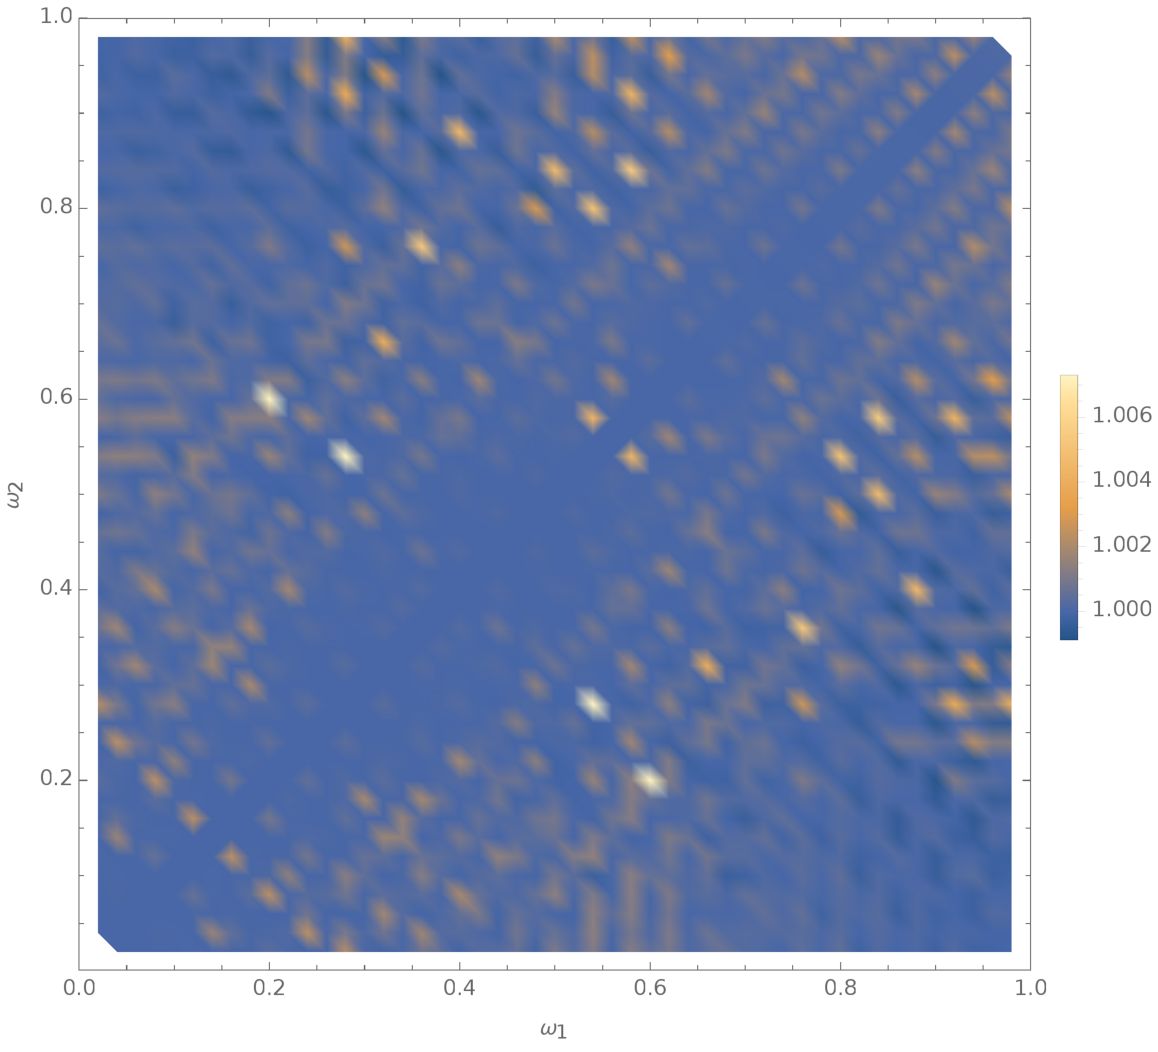
\includegraphics[width=0.6\textwidth]{plot/energy-ratio-sine-1d.pdf}
  \caption{Values of $E/E_{\rm init}$ for 1D sine-Gordon. They are necessarily 1 as 1D sine-Gordon oscillons do not leak energy.}\label{sine1denergy}
\end{figure}

We will use three numerical metrics to assess whether oscillons with two-scale features are present in more general potentials and dimensionalities.  The first is the fraction of the initial energy contained within a resulting oscillon --- if this fraction is small,  the resulting solution likely has little in common with initial state, as the majority of the energy supplied by the initial configuration has  been radiated away. Recall that the energy density is:
\begin{equation}
  e(t,r) = \frac{1}{2}\left(\phi_t^2+ \nabla \phi\cdot \nabla \phi \right) + V(\phi) \, .
\end{equation}
The numerical integrator will integrate the energy density within a given box $r_0$ and produce the percentage of the total energy within the box at the end of the simulation compared to the start, which will be denoted by $E/E_{\rm init}$.

The second qualitative criterion assesses the existence and stability of the off-centered peaks. For this purpose we will use
\begin{equation}
  \langle r_{\rm max} \rangle  = \left\langle \argmax_{r < r_0} |\phi(t,r)| \right\rangle_t
\end{equation}
which is the time average of the peak radius. A non-zero value indicates an off-centered peak that exists for a sufficiently long time. We will ignore outgoing radiations by only considering the field values within a radius $r_0$.

The numerical metric indicates the ``strength'' of the breathing behaviours we described earlier. To this end, we will look at the field values at the origin which, if the oscillon is breathing, will have a slow mode superimposed on the fast mode. We will use the average period of the slow mode multiplied by the average amplitude to indicate the ``strength'' of the breathing behaviour. We will denote this quantity by $S$.

It is instructive to look at these three numerical metrics for the exact two-scale solution for 1D sine-Gordon. The quantity $E/E_{\rm init}$ will necessarily be 1, as the oscillons are stable and live infinitely long, and therefore do not produce any energy loss through radiation. This is validated in Fig.~\ref{sine1denergy}.

\begin{figure}
  \centering
  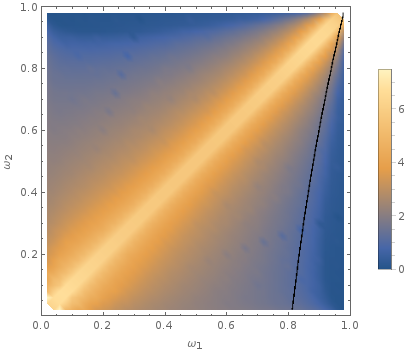
\includegraphics[width=0.45\textwidth]{plot/r_max-sine-1d.png}
  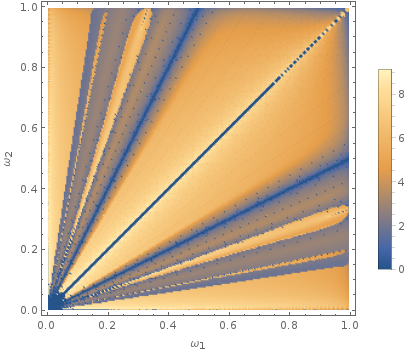
\includegraphics[width=0.45\textwidth]{plot/slow-mode-sine-1d.png}
  \caption{Values $\langle r_{\rm max}\rangle$ (upper) and  $\log{S}$ (lower) for 1D sine-Gordon.}\label{sine-1d}
\end{figure}

Next we look at the values of $\langle r_{\rm max}\rangle$ and $\log{S}$ for 1D sine-Gordon, which are plotted in Fig.~\ref{sine-1d}. The plot of $\langle r_{\rm max}\rangle$ indicates that there is a region in the parameter space, near $\omega_1=1$, where the peak displacement disappear and the oscillons are singly peaked. This is consistent with our analytical result in (\ref{disp}): if one plots the line where the inside of the $\cosh^{-1}$ goes below 1, thus rendering $x_d$ imaginary, one obtains the same boundary line in the dark-coloured region of the $\langle r_{\rm max}\rangle$ plot in Fig.~\ref{sine-1d}.

The $\log S$ plot for 1D sine-Gordon indicates that near the diagonal line, as well as the lower triangle in the parameter space, there are stronger breathing modes than other regions. The fact that the region near the diagonal line has strong breathing modes is explained by the interference of two single-scale oscillon, as is the case in the linear theory. The triangular region near the bottom has large $\log S$ because of the exotic behaviours in the large-amplitude limit.

\begin{figure}[p]
  \begin{adjustwidth}{-1in}{-1in}
    \centering
    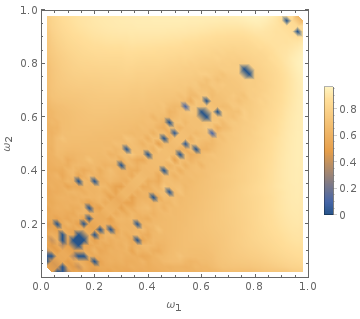
\includegraphics[width=0.45\textwidth]{plot/energy-ratio-axion-1d.png}
    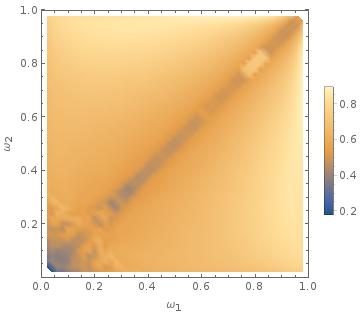
\includegraphics[width=0.45\textwidth]{plot/energy-ratio-axion-2d.png}
    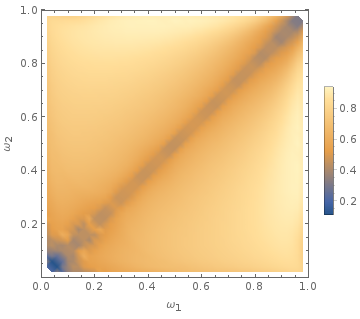
\includegraphics[width=0.45\textwidth]{plot/energy-ratio-axion-3d.png} \\
    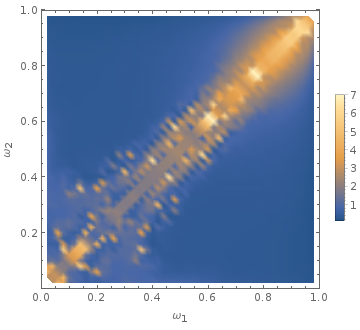
\includegraphics[width=0.45\textwidth]{plot/r_max-axion-1d.png}
    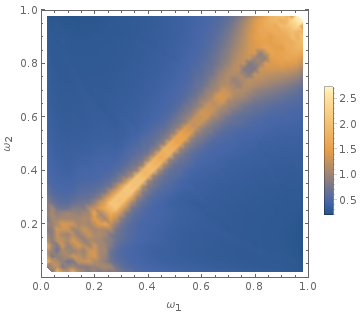
\includegraphics[width=0.45\textwidth]{plot/r_max-axion-2d.png}
    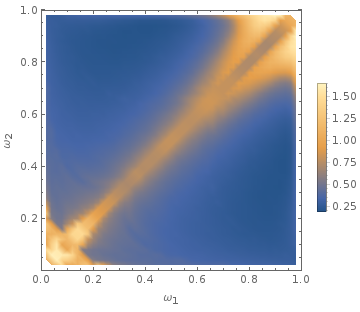
\includegraphics[width=0.45\textwidth]{plot/r_max-axion-3d.png} \\
    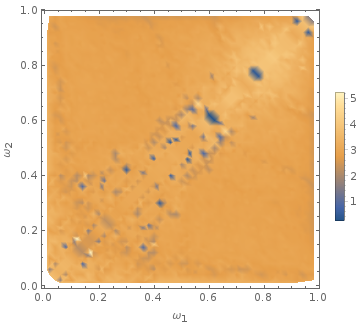
\includegraphics[width=0.45\textwidth]{plot/slow-mode-logscale-axion-1d.png}
    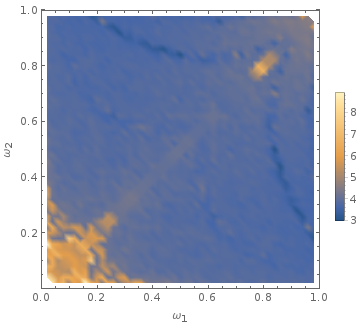
\includegraphics[width=0.45\textwidth]{plot/slow-mode-logscale-axion-2d.png}
    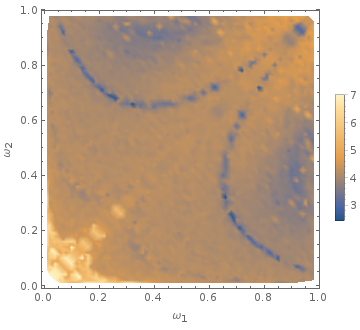
\includegraphics[width=0.45\textwidth]{plot/slow-mode-logscale-axion-3d.png}
    \caption{Qualitative properties of pulsating oscillon solutions for the axion monodromy potential. Top row: $E/E_{\rm init}$ at $t=4000$.
      Middle row: $\langle r_{\rm max}\rangle$.
      Bottom row: Strength of slow modes, $\log{S}$.\quad
      Left to right: 1D, 2D, 3D. We see that 50\% of the initial energy typically remains in the oscillon, and the peak is displaced furthest from the origin when $\omega_1 \approx \omega_2$. All choices of  $\omega_1$ and $\omega_2$ lead to a pulsating envelope, which is most pronounced when $\omega_1$ and $\omega_2$ are small in 2D and 3D. The ``holes'' in the 1D solution are associated with cases where the initial profile splits into two single oscillons moving away from the origin.}\label{axion-monodromy}
  \end{adjustwidth}
\end{figure}

\section{Axion-monodromy Potential}
We computed the three numerical metrics for the axion-monodromy potential (\ref {axion-potential}) in 1, 2, and 3 spatial dimensions. The reason that we wish to study this potential is that it is a natural candidate for the inflaton field and has provided a physical example where the post-inflationary universe may be dominated in axion-monodromy oscillons (see Section \ref{litrev:cosmo} and Chapter \ref{appcosmo}). 

As can be seen in Fig.~\ref{axion-monodromy}, in almost all regions of the parameter space, we see that the axion-monodromy oscillons initialized with the exact two-scale solution retain $>50\%$ of their initial energies. This means that the axion-monodromy two-scale oscillons share a reasonable similarity with the two-scale 1D sine-Gordon oscillons in terms of their field dynamics, quantified by the fact that a significant portion of the initial energy stays within the oscillon and does not radiate out when settling into the stable, attractor point oscillon configuration. This enables us to model the axion-monodromy oscillons that we have obtained in the early universe simulation with the ansatz provided by the exact 1D sine-Gordon solution, which we will take up in Chapter \ref{appcosmo}.

For the $\langle r_{\rm max}\rangle$ and $\log S$ values, we see a similar dependence on $(\omega_1,\omega_2)$ parameters to the 1D sine-Gordon case: significant pulsations were observed in the most of the $(\omega_1,\omega_2)$ space.
 
\section{Sine-Gordon Potential in 2 and 3D}

We plot the three qualitative measures for the sine-Gordon potential in 2D and 3D in Fig.~\ref{sine2d3d}. From the $\langle r_{\rm max}\rangle$ and $\log{S}$, as well as from examining the field evolution directly, we find that there exist long-lived, pulsating oscillons in 2D sine-Gordon (in agreement with  \cite{Hindmarsh:2006ur}). However, from the energy conservation heat-map the $E/E_{\rm init}$ is much less than unity, suggesting these oscillons are less closely related to their exact 1D analogues. In 3D, our initial ansatz does not yield stable oscillons over most of the $(\omega_1,\omega_2)$ plane.

\begin{figure}[p]
  \centering
  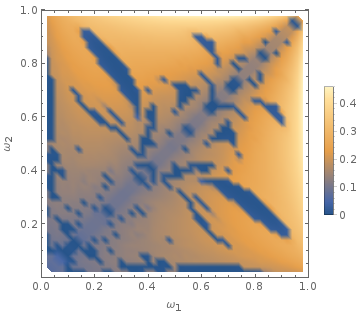
\includegraphics[width=0.45\textwidth]{plot/energy-ratio-sine-2d.png}
  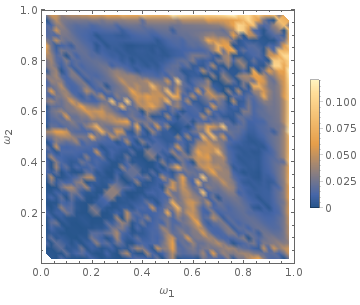
\includegraphics[width=0.45\textwidth]{plot/energy-ratio-sine-3d.png} \\
  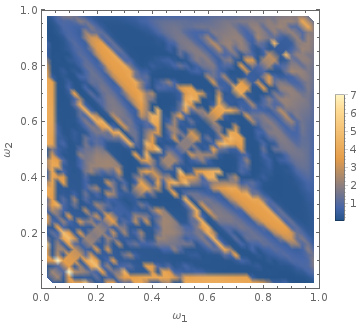
\includegraphics[width=0.45\textwidth]{plot/r_max-sine-2d.png}
  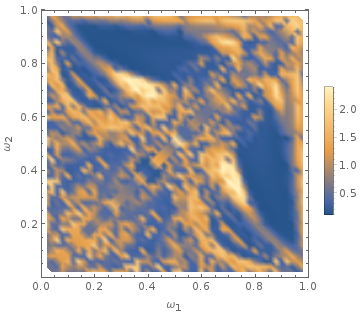
\includegraphics[width=0.45\textwidth]{plot/r_max-sine-3d.png} \\
  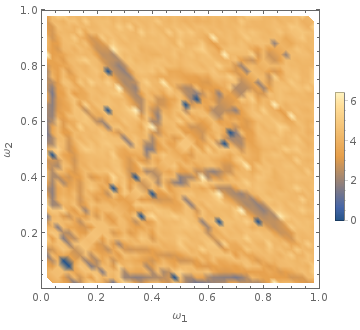
\includegraphics[width=0.45\textwidth]{plot/slow-mode-logscale-sine-2d.png}
  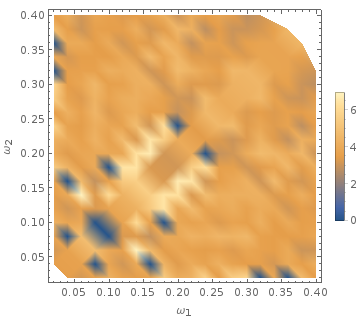
\includegraphics[width=0.45\textwidth]{plot/slow-mode-logscale-sine-3d.png}
  \caption{Qualitative properties of pulsating oscillon solutions for the sine-Gordon potential. Top row: $E/E_{\rm init}$ at $t=4000$.
    Middle row: $\langle r_{\rm max}\rangle$.
    Bottom row: Strength of slow modes, $\log{S}$.\quad
    Left to right: 2D, 3D.\qquad From the energy conservation heat-map, we find that pulsating oscillons in 2D sine-Gordon share less similarity with the exact 1D sine-Gordon solutions. For 3D sine-Gordon, the oscillons starting from the two-scale ansatz are not stable.}\label{sine2d3d}
\end{figure}

\section{$\phi^6$ Potential}
For the $\phi^6$ potential, we find that when $g$ is small, it supports pulsating oscillons in 1, 2 and 3D near the $(1,1)$ corner of the parameter space (see Fig.~\ref{phi6}). As $g$ goes larger, the region which supports oscillons becomes smaller and smaller. For large $g$, two-scale oscillons exist only if  $\omega_1$ and $\omega_2$ are extremely close to unity. What we have shown in Fig.~\ref{phi6} is a moderate value $g=1$ for which a reasonably substantial region of the parameter space supports two-scale oscillons.

\begin{figure}[p]
  \begin{adjustwidth}{-1in}{-1in}
    \centering
    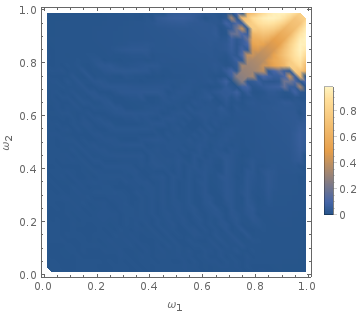
\includegraphics[width=0.45\textwidth]{plot/energy-ratio-phi6-1d.png}
    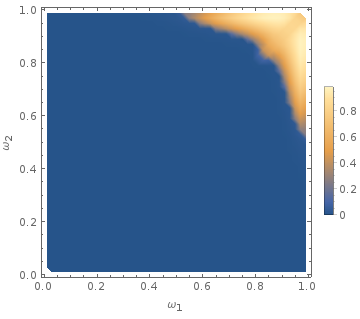
\includegraphics[width=0.45\textwidth]{plot/energy-ratio-phi6-2d.png}
    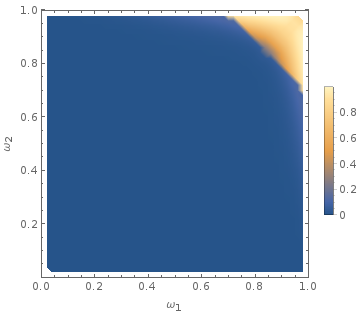
\includegraphics[width=0.45\textwidth]{plot/energy-ratio-phi6-3d.png} \\
    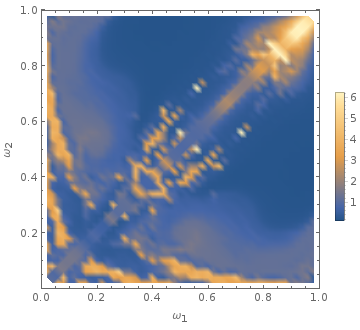
\includegraphics[width=0.45\textwidth]{plot/r_max-phi6-1d.png}
    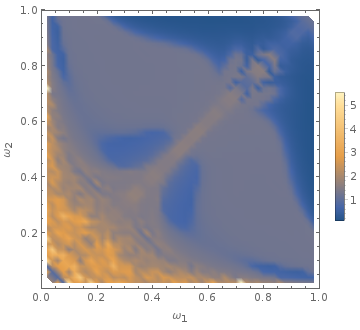
\includegraphics[width=0.45\textwidth]{plot/r_max-phi6-2d.png}
    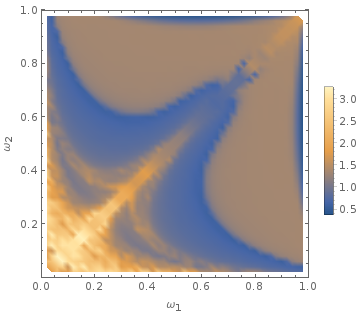
\includegraphics[width=0.45\textwidth]{plot/r_max-phi6-3d.png} \\
    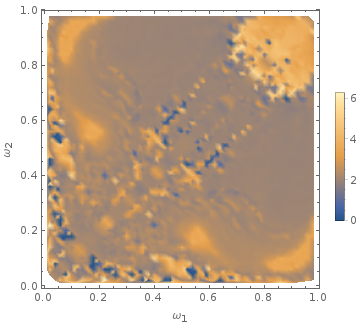
\includegraphics[width=0.45\textwidth]{plot/slow-mode-logscale-phi6-1d.png}
    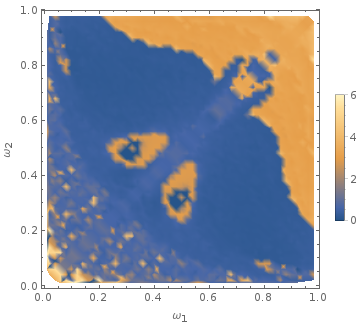
\includegraphics[width=0.45\textwidth]{plot/slow-mode-logscale-phi6-2d.png}
    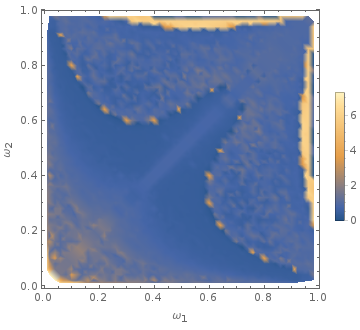
\includegraphics[width=0.45\textwidth]{plot/slow-mode-logscale-phi6-3d.png}
    \caption{Qualitative properties of pulsating oscillon solutions for the $\phi^6$ potential with $g=1$. Top row: $E/E_{\rm init}$ at $t=4000$.
      Middle row: $\langle r_{\rm max}\rangle$.
      Bottom row: Strength of slow modes, $\log{S}$.\quad
      Left to right: 1D, 2D, 3D. \qquad What we have shown here is a moderate value of $g$, where a reasonably substantial region of the parameter space supports two-scale oscillons. If $g$ is significantly larger than $1$, the region which supports two-scale oscillons will be diminishingly small.}\label{phi6}
  \end{adjustwidth}
\end{figure}

\chapter{Application to Axion-Monodromy Inflation}\label{appcosmo}

In this Chapter, we will apply the results in the previous two Chapters, which state that, in particular, the axion-monodromy oscillons in 3D have a reasonably good overlap with the exact two-scale solutions, to the oscillons in the numerical simulation of the post-inflationary universe. The literature that we have reviewed in Section \ref{litrev:cosmo} suggest that parametric resonance can generate an oscillon-dominated phase in the (p)re-heating stage of the inflationary universe. We will use PSpectRE \cite{Easther:2010qz} to simulate the axion-monodromy inflaton field within a homogeneous expanding universe, and evolve the field dynamics to obtain an oscillon-dominated universe. We will then cut out the oscillon profiles from the simulated universe through a series of post-processing procedures on the raw simulated data. From the numerical oscillon profiles, we will use an ansatz obtained from the small-amplitude limit of the exact two-scale solution to obtain an analytic fit, and observe that the analytic model gives a tolerable fit to many, but not all, of the simulated oscillons in the early universe.

\section{PSpectRE and the Simulation Settings}
PSpectRE \cite{Easther:2010qz} is a Fourier-space pseudo-spectral methods that simulates interacting scalar fields in an expanding universe. It is written in C++ and can optionally target OpenMP to utilize the multi-core capability of a modern CPU. The simulation settings, as well as the full source code that we used in this project are available in \cite{pspectregh}.

A representative time-slice of the oscillon-dominated phase in the simulated universe is shown in Fig.~\ref{oscillons}. The diagram represents the contour plot of the energy density of the axion-monodromy inflaton field. The orange blobs in the diagram are regions with individual oscillons, and are surfaces of equal energy density, and the gray contours are equal-density contours of 4 times the energy density on the surface of the oscillons.

We have plotted the field value at the center of a particular oscillon in the simulation in Fig.~\ref{raw}. As can be seen in this diagram, in general, the oscillons from our simulation have strong breathing modes with more complex dynamics than can be fully encoded with the two-scale solution. Nonetheless, we can use the two-scale solution to achieve a reasonably good fit for many of the oscillons from simulation, accounting for most of the local breathing dynamics but not necessarily global, long-term evolution.

The oscillons from the PSpectRE simulations do not have off-center peaks, as can be seen in Fig.~\ref{oscillons}.

\begin{figure}
  \centering
  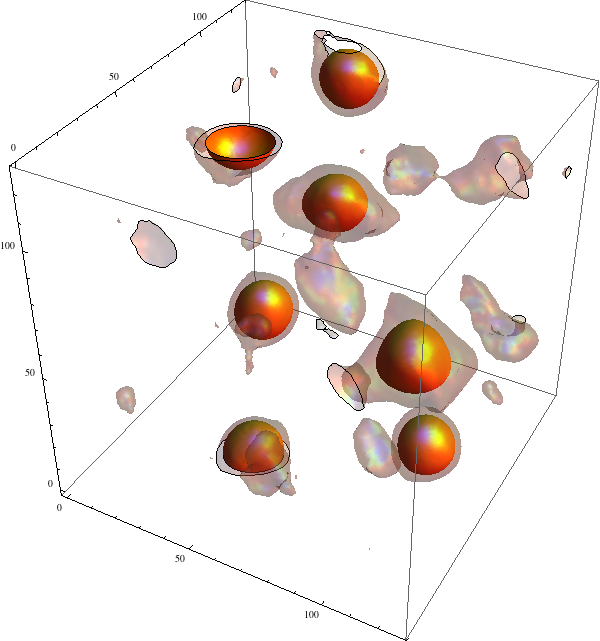
\includegraphics[width=0.6\textwidth]{plot/3dRE.png}
  \caption{Oscillons following monodromy inflation  \cite{Easther:2010qz}. Contours show regions of mean and 4 $\times$ mean density. }\label{oscillons}
\end{figure}

\begin{figure}
  \centering
  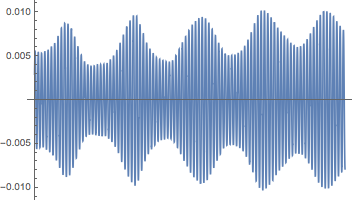
\includegraphics[width=0.7\textwidth]{plot/3Doscillon.png} 
    \caption{Central value of an oscillon extracted from full 3D numerical solution.}
  \label{raw}
\end{figure}

\subsection{Side-quest: Porting PSpectRE to CUDA}
The original PSpectRE code targets OpenMP for accelerating the vector operations that comprise the bulk of the computations done in the simulation. Due to their highly parallelizable nature, these vector operations are an ideal candidate for parallelizing using the GPU. A modern GPU can spawn thousands of threads in parallel, while in comparison a typical desktop CPU has only four processor cores. Therefore, porting PSpectRE to the GPU will theoretically result in a huge speed-up, if done correct so that the new code respects the memory and processing model of the GPU, which has significant differences from the ordinary CPU computing model.

In running the simulations during this project, the original PSpectRE code has seen limitations when it comes to computation speed. It was therefore deemed profitable to spend some time porting the PSpectRE code into the GPU, in anticipation of the relatively numerous simulations that would be done. The relevant portion of the PSpectRE code has now been ported to the CUDA computing platform which targets modern NVidia GPU's, and is available at \cite{cudaport}.

Note that only the features that are required in this project have been ported to CUDA. The rest of the functions have been stripped from the code-base to simplify the porting process. It is, however, a relatively trivial matter to port the rest of the features over, as they are simple vector operations that share great similarity with each other.

\section{The Small-amplitude Limit}
It is possible to derive an approximate expression for the two-scale solution, valid for the region of the parameter space that contains the numerical axion-monodromy oscillons. This approximate solution will be used as an ansatz to fit the numerical oscillon profiles in the next Section. For the full solution eqs.~(\ref{twoscale})--(\ref{denomg}), we first notice that when $\omega_1\approx\omega_2$, we have
\begin{equation}
  \frac{\omega_1^2+\omega_2^2}{\omega_1 \omega_2} \approx 2
\end{equation}
and likewise for $r_i$. We can therefore collect the $\cos$ and $\cosh$ terms in the denominator eq.~(\ref{denomf}) and (\ref{denomg}) into one single term:
\begin{equation}
  f(t) \approx \cos (\omega_1-\omega_2) t
\end{equation}
and
\begin{equation}
  g(x) \approx \cosh (r_1-r_2) x
\end{equation}

For the numerator, we will use the trigonometric identity
\begin{equation}
  a\cos x + b \cos(x+\theta) = c \cos(x+\phi)
\end{equation}
where
\begin{equation}
  c = \sqrt{a^2+b^2+2ab\cos\theta}
\end{equation}
and
\begin{equation}
  \phi=\arctan \frac{b\sin\theta}{a+b\cos\theta}
\end{equation}

To simplify the notation and reflect the fact that $\omega_1$ and $\omega_2$ are close to each other, we set $\omega=\omega_1$ and $\delta=\omega_1-\omega_2>0$. Note that when both $\omega_i\to1$, we necessarily have $\delta\to0$, and $r_1-r_2\approx \omega \delta/\sqrt{1-\omega^2}$.

The numerator is then proportional to
\begin{equation}
  \sqrt{2\cosh^2 rx + 2\cosh^2 (rx) \cos(\delta t)}\cos(\omega t+\phi)
\end{equation}
where $\phi = -\delta t/2$ and therefore $\cos(\omega t+\phi)=\cos((\omega_1+\omega_2)t/2)\approx\cos\omega t$.

The full solution then becomes
\begin{equation}\label{approxexpr}
  u(t,x) \approx 8\sqrt{2}  \frac{\delta}{\sqrt{1-\omega^2}} \sqrt{1+\cos\delta t} \cos\omega t \frac{\cosh \sqrt{1-\omega^2} x}{\cosh(\omega\delta x/\sqrt{1-\omega^2}) + \cos \delta t}
\end{equation}

For this approximate expression to apply we need $(1-\omega^2)/\omega < \delta$. Otherwise, the denominator in  (\ref{approxexpr}) goes to 0, and the expression goes to infinity.

\section{Fitting against the Two-scale Solution}

\begin{figure}
  \centering
  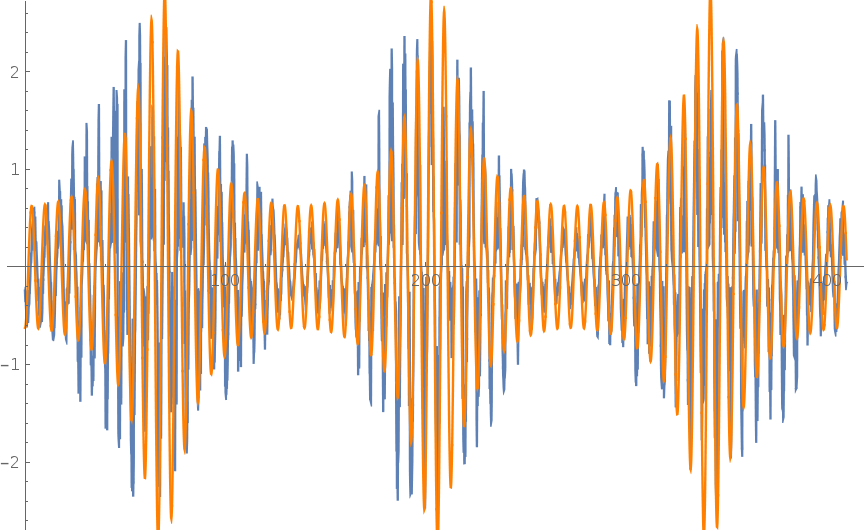
\includegraphics[width=0.8\textwidth]{plot/simul-profile.png}
  \caption{[Blue] Field value at the center of an oscillon from 3D monodromy simulation. [Orange] Fitted profile eq.~(\ref{fitprof}); $A=0.863$, $\omega=0.946$, $\epsilon=0.91$,  $\delta=0.046$.}\label{simul-prof}
\end{figure}

From (\ref{approxexpr}), we can generalize the approximate expression to obtain an ansatz that captures the essential, local dynamics of the numerical axion-monodromy oscillons. We will absorb the constant term $8\sqrt{2}  \delta/\sqrt{1-\omega^2}$ in front of the expression inside the $\arctan$ function into the amplitude parameter $A$, and the term $\sqrt{1-\omega^2}/\omega\delta$ inside the $\cosh$ term in the denominator into the width parameter $R$. We also note that as $\omega\to1$, the term in the numerator $\cosh\sqrt{1-\omega^2} x\to1$, and may therefore be set it to 1. The approximate solution then becomes
\begin{equation}
  u(t,x) \approx A \cos\omega t \frac{\sqrt{1+\cos\delta t} }{\cosh(x/R) + \cos \delta t}  
\end{equation}

In order to account for the different breathing mode amplitudes in the simulated oscillons, and to remove the singularity introduced by the approximation, we will add a new adjustable parameter $\epsilon$, which will serve as the breathing mode amplitude. We will also switch the spatial variable to $r$ to account for the fact that we have assumed spherical symmetricity. The final form of our analytic ansatz is then
\begin{equation} \label{fitprof}
  u(t,r) = A\cos\omega t \frac{\sqrt{1+\epsilon \cos \delta t}}{\cosh(r/R) + \epsilon \cos \delta t}
\end{equation}
where $\epsilon<1$ and $\delta = \omega_1-\omega_2 \ll 1$. This provides an analytical template against which the numerical axion-monodromy oscillon profiles are fitted.

We have plotted the original oscillon profile extracted from the 3D monodromy inflation, and the fitted profile in Fig.~\ref{simul-prof}. As can be seen from the diagram, the analytic ansatz has provided a tolerable fit of the local breathing dynamics of the simulated oscillon, spanning about three slow-mode periods. For longer-time dynamics, this simple ansatz will need to be extended to account for the complex global dynamics, possibly through an adiabatic evolution of the fitted parameter $A$, $R$, $\delta$, and $\epsilon$, which we have assumed to be constant in this simple model.

\begin{figure}
  \centering
  \includegraphics[width=0.8\textwidth]{plot/profile-3scale.png}
  \caption{Spherically symmetric 3D monodromy oscillon initialized with 1D
    sine-Gordon profile $\omega_1=0.999$, $\omega_2=0.950$.}\label{threescales}
\end{figure}

\begin{figure}
  \centering
  \includegraphics[width=0.8\textwidth]{plot/fourier.png}
  \caption{Fourier spectrum. Inset shows peaks around the dominant mode $\omega_0\approx0.95$.}\label{fourier}
\end{figure}

One might wonder if some of the longest-period modulations are induced by the oscillon's interaction with its environment, or finite resolution effects in a 3D code, or the overall expansion of the universe. However, similar oscillon solutions are seen in the spherically symmetric code initialized with a 1D sine-Gordon profile with one of the $\omega_i\to1$ (see Fig.~\ref{threescales}). Ref.~\cite{Salmi:2012ta} previously investigated 3D oscillons in a monodromy-like potential initialized with a Gaussian profile. For these solutions the Fourier spectrum of $u(t,0)$ has several distinct peaks, but the dominant mode has $\sim 100\times$ more power than the next highest peaks. The corresponding spectrum seen here is far more complex,  as can be seen from  Fig.~\ref{fourier}. The overall energy of these oscillons can decrease abruptly, suggesting that on long timescales the solutions are aperiodic.

\chapter{Stability Analysis}

Despite being not applicable to the axion-monodromy potential, the non-pertur\-bative method in \cite{PhysRevD.80.125037, Gleiser:2008ty} can nonetheless correctly explain the oscillon stability in polynomial potentials. Since we have seen that various numerical studies (see discussions in Section \ref{nonpert}) indicate that there is a proliferation of breathing oscillons near the stable-unstable boundary (see Fig.~\ref{stability}), it is instructive to perform the same stability analysis in \cite{PhysRevD.80.125037, Gleiser:2008ty} with the two-scale ansatz for the breathing oscillons. We will see that the new breathing ansatz extends the region of stability near the stable-unstable boundary, at least for polynomial potentials where the non-perturbative method in \cite{PhysRevD.80.125037, Gleiser:2008ty} is applicable.

We perform essentially the same procedure in eqs.~(\ref{lagfull}) to (\ref{effpot}), but with the following ansatz derived from (\ref{fitprof}):
\begin{equation}
  u(t,r) = A(t)\,\frac{\sqrt{1+d\,}}{\cosh r/R + d\,}
\end{equation}
with $d<1$. We have replaced $\epsilon\cos\delta t$ with $d$, in order to simplify the model. The justification for this is that $\delta\to 0$ compared to $\omega\approx 1$, and therefore contributes less to the dynamics.

For a $\phi^4$ model with
\begin{equation}
  V(\phi) = \phi^2 - \phi^3 + \frac{\phi^4}{4}
\end{equation}
we obtain the following stability criterion
\begin{equation}
  I(A,R,d) = V_{\rm eff}''(A) = f_{01}(A,R,d) + f_3(A,R,d) + f_4(A,R,d)
\end{equation}
where
\begin{equation}
  f_{01}(A,R,d)=A^2\frac{\left(11 d^2+4\right) \sqrt{1-d^2}-6 d \left(2 d^2+3\right) \arctan\sqrt{\frac{1-d}{1+d}}}{2 (1-d)^2 (d+1) \left(\sqrt{1-d^2}
      -2 d \arctan\sqrt{\frac{1-d}{1+d}}\right)}
\end{equation}
and
\begin{equation}
  f_3(A,R,d)=3A\frac{3 d \sqrt{1-d^2}-2 \left(2 d^2+1\right) \arctan\sqrt{\frac{1-d}{1+d}}}{(1-d)^{3/2} (d+1) \left(1-\frac{2 d \arctan\sqrt{\frac{1-d}{1+d}}}{\sqrt{1-d^2}}\right)}
\end{equation}
and
\begin{equation}
    f_4(A,R,d)=2 \left(1+\frac{d^2-\frac{6 d \arctan\sqrt{\frac{1-d}{1+d}}}{\sqrt{1-d^2}}+2}{24 (1-d) (d+1) R \left(1-\frac{2 d \arctan\sqrt{\frac{1-d}{1+d}}}{\sqrt{1-d^2}}\right)}\right)
\end{equation}
We then plot the stability curves in Fig.~\ref{stability1}.

\begin{figure}\centering
  \includegraphics[width=0.6\textwidth]{plot/small-stability.png}
  \caption{$A$-$R$ diagram (horizontal axis is $A$). Dashed line is $d=0$ (ie.~no breathing modes). Blue line is $d=-0.6$. Orange line is $d=0.6$.}\label{stability1}
\end{figure}

We see from Fig.~\ref{stability1} that the option of having a breathing mode slightly increases the area of stable oscillons, and these breathing modes appear in the boundary of stability curve in the $A$-$R$ diagram (the common area inside both the blue curve and the orange curve), which is consistent with our numerical results discussed in Section \ref{nonpert}.

A problem with carrying out the same analysis to the axion monodromy case, in addition to the previously mentioned problem in Chapter \ref{nonpertprob}, is that with the new ansatz, the integral with the axion-monodromy potential can no longer be performed analytically.

\chapter{Conclusion}

In this Thesis, we reviewed the vast literature from applied mathematics and physics that are dedicated to the study of oscillon dynamics in classical scalar field theories. We then pointed out the limitations of previous studies in terms of accounting for the breathing behaviours in axion-monodromy oscillons, which prompted us to search for a more complex oscillon solution with two time-scales.

Utilizing the integrability of the 1D sine-Gordon equation, we derived the exact two-scale solution, and numerically extend this result to more general potentials and dimensionalities. We observed that the breathing modes and off-center peaks in the field dynamics of the exact solution are still present in more general settings, which suggests that the exact two-scale solution can be used to model oscillon behaviours in more complex potentials.

Finally, we applied our mathematical results to the axion-monodromy oscillons in the post-inflationary universe, and concluded that the analytic ansatz from the exact solution can account for local, but not global, breathing dynamics of the axion-monodromy oscillons from the early-universe simulations.

\bibliographystyle{plain}
\bibliography{references}

\end{document}
